\documentclass[11pt,aspectratio=169]{beamer}

\usepackage[T1]{fontenc}
\usepackage{lmodern}
\usepackage{graphicx}
\usepackage{tikz}
\usetikzlibrary{arrows.meta,positioning,calc,decorations.pathreplacing,overlay-beamer-styles,shapes.geometric,patterns}
\usepackage{pgfplots}
\pgfplotsset{compat=1.17}
\usepackage{amsmath,amssymb,mathtools}
\usepackage{booktabs,tabularx,array,multirow}

\setbeamercovered{transparent=5}
\setbeamertemplate{navigation symbols}{}
\setbeamertemplate{itemize items}[circle]
\setbeamertemplate{itemize subitem}{--}
\setbeamertemplate{footline}[frame number]
\setbeamerfont{framesubtitle}{size=\small}
\setbeamercolor{block title}{fg=black,bg=white!80!black}
\setbeamercolor{block body}{fg=black,bg=white!97!black}
\linespread{1.2}
\setbeamersize{text margin left=0.5cm,text margin right=0.5cm}

\newcommand{\1}{\mathbf 1}
\newcommand{\E}{\mathbb E}
\newcommand{\takeaway}[1]{\vfill{\small\textbf{Takeaway.} #1}}

\begin{document}

%--------------------------------------------------------------------
\begin{frame}[t]{Tenure Segmentation and the Space Floor}
\linespread{1.0}\selectfont\vspace{-0.5em}
\noindent{\footnotesize Within a period a renter with $m$ children at home splits expenditure $x = c + r h^R$ between consumption $c$ and rental space $h^R$ at rent $r$ per room; the uncapped optimum is $h^{R*}_m(x) = (1-\alpha)x/r + \alpha m h_P$, where $h_P$ is the parenthood space floor and $\alpha = 0.733$ the consumption share.}

\vspace{-0.4em}
\begin{minipage}[t]{0.535\textwidth}
\vspace{0pt}
\centering
\begin{tikzpicture}
\begin{axis}[
  width=\linewidth, height=0.50\textheight,
  xmin=0, xmax=4.2, ymin=0, ymax=10,
  xtick={0,1,2.16,3.16,4}, xticklabels={0,1,$x_1$,$x_0$,4},
  ytick={0,2,4,6,8,10},
  xlabel={\scriptsize expenditure $x = c + r h^R$ (per period)},
  ylabel={\scriptsize desired space (rooms)},
  tick label style={font=\scriptsize},
  label style={font=\scriptsize},
  clip=true, axis line style={black}
]
% owned-only region above the cap
\fill[pattern=north east lines, pattern color=gray!45] (axis cs:0,6) rectangle (axis cs:4.2,10);
% band between x_1 and x_0
\fill[gray, opacity=0.25] (axis cs:2.16,0) rectangle (axis cs:3.16,6);
\draw[gray!70] (axis cs:2.16,0) -- (axis cs:2.16,6);
\draw[gray!70] (axis cs:3.16,0) -- (axis cs:3.16,6);
% desired-space lines
\addplot[thick, domain=0:4.2, samples=2] {1.90*x};
\addplot[thick, domain=0:4.2, samples=2, color=blue!70!black] {1.90*x+1.90};
% cap and floor
\draw[very thick] (axis cs:0,6) -- (axis cs:4.2,6);
\draw[dashed] (axis cs:0,2.6) -- (axis cs:4.2,2.6);
% crossing points
\fill (axis cs:2.16,6) circle (1.4pt);
\fill (axis cs:3.16,6) circle (1.4pt);
% owner menu
\fill (axis cs:4.2,2) circle (1.6pt); \fill (axis cs:4.2,4) circle (1.6pt); \fill (axis cs:4.2,6) circle (1.6pt); \fill (axis cs:4.2,8) circle (1.6pt); \fill (axis cs:4.2,10) circle (1.6pt);
% labels
\node[anchor=north west, font=\tiny, inner sep=1pt] at (axis cs:0.08,5.95) {rental cap $\bar h^R$};
\node[anchor=north east, font=\tiny, inner sep=1pt] at (axis cs:4.1,2.55) {space floor $h_P$};
\node[anchor=north west, font=\tiny, inner sep=1pt, text width=1.4cm] at (axis cs:3.3,5.2) {childless $h^{R*}_0(x)$};
\node[anchor=south east, font=\tiny, inner sep=1pt, text width=1.6cm, align=right, color=blue!70!black] at (axis cs:3.1,8.0) {one child at home $h^{R*}_1(x)$};
\node[font=\tiny, inner sep=1pt, text width=1.7cm, align=center] at (axis cs:2.66,1.1) {parents capped, childless not};
\node[anchor=east, font=\tiny, inner sep=1pt] at (axis cs:4.05,0.9) {owner menu};
\node[font=\tiny, inner sep=2pt, text width=2.6cm, align=center, fill=white, fill opacity=0.85, text opacity=1] at (axis cs:0.78,8.0) {owned units only: 8 or 10 rooms; equity $(1-\phi)Ph$ built from consumption-savings};
\end{axis}
\end{tikzpicture}
\end{minipage}\hfill
\begin{minipage}[t]{0.445\textwidth}
\vspace{0pt}
\linespread{1.0}\scriptsize\setlength{\leftmargini}{1em}
\begin{itemize}\setlength{\itemsep}{0.2em}\setlength{\parskip}{0pt}
\item Segmentation $=$ floor plus cap: a parent's desired rental space crosses the cap $\bar h^R = 6$ at $x_1 = r(\bar h^R - \alpha h_P)/(1-\alpha)$, a childless household's at $x_0 = r\bar h^R/(1-\alpha) > x_1$.
\item On $(x_1, x_0)$ only the parent is rationed; extra space exists only in the owner menu, so the family-space option depends on ownership access: liquid wealth, income this period, housing equity.
\item At the benchmark ($r = 0.141$, $h_P = 2.6$): $x_1 \approx 2.16$, $x_0 \approx 3.16$ per four-year period; a median lower-middle-income renter spends $x \approx 2.58$, wants 4.9 rooms childless and 6.8 rooms as a parent.
\end{itemize}
\end{minipage}

\takeaway{Children raise desired space by $\alpha h_P \approx 1.9$ rooms at any budget; the cap turns that into a tenure question for lower-middle-income renters.}
\end{frame}

%--------------------------------------------------------------------
\begin{frame}[t]{Rationed Space and Income Risk: Theory and Full-Model Check}
\linespread{1.0}\selectfont\vspace{-0.6em}
{\scriptsize Let $J^{\infty}_1(x)$ and $J^{\bar h}_1(x)$ be a parent's value of expenditure $x$ without and with the rental cap, and $L = J^{\infty}_1 - J^{\bar h}_1 \ge 0$ the loss from the cap: $L = 0$ for $x \le x_1$ and $L''(x_1^+) = \frac{1-\alpha}{\alpha}\,\frac{\lambda}{x_1 - r h_P} > 0$ ($\lambda$: marginal utility of expenditure). Risk around $x_1$ costs a parent more than a childless household.\par}\vspace{-0.2em}

\vspace{-0.3em}
\begin{minipage}[t]{0.36\textwidth}
\vspace{0pt}
\centering
\begin{tikzpicture}
\begin{axis}[
  width=1.08\linewidth, height=0.38\textheight,
  xmin=1.4, xmax=3.0, ymin=-0.012, ymax=0.17,
  xtick={2.16}, xticklabels={$x_1$}, ytick=\empty,
  xlabel={\scriptsize expenditure $x$},
  ylabel={\scriptsize loss $L(x)$},
  tick label style={font=\scriptsize},
  label style={font=\scriptsize},
  axis lines=left, clip=true
]
\addplot[thick, domain=1.4:2.16, samples=2] {0};
\addplot[thick, domain=2.16:3.0, samples=60] {0.2*(x-2.16)^2};
\draw[dashed] (axis cs:1.76,0) -- (axis cs:2.56,0.032);
\draw[dotted, gray] (axis cs:2.16,-0.012) -- (axis cs:2.16,0.016);
\fill (axis cs:1.76,0) circle (1.4pt);
\fill (axis cs:2.56,0.032) circle (1.4pt);
\fill[red!70!black] (axis cs:2.16,0.016) circle (1.8pt);
\node[anchor=south, font=\tiny, inner sep=1pt] at (axis cs:1.76,0.005) {$\bar x - \varepsilon$};
\node[anchor=north west, font=\tiny, inner sep=1pt] at (axis cs:2.58,0.03) {$\bar x + \varepsilon$};
\node[anchor=south west, font=\tiny, inner sep=1pt, text width=2.2cm] at (axis cs:1.42,0.05) {$\E L(X) > L(\bar x) = 0$ for $X=\bar x\pm\varepsilon$, $\bar x = x_1$};
\draw[->, red!70!black] (axis cs:1.95,0.048) -- (axis cs:2.13,0.02);
\node[anchor=south east, font=\tiny, inner sep=1pt, text width=2.0cm, align=right] at (axis cs:2.85,0.115) {parents cannot expand space in good states};
\end{axis}
\end{tikzpicture}
\end{minipage}\hfill
\begin{minipage}[t]{0.62\textwidth}
\vspace{0pt}
\scriptsize\setlength{\leftmargini}{1em}
\textbf{Full-model check (fixed price, matched states, ages 22--33)}
\begin{itemize}\setlength{\itemsep}{0.1em}\setlength{\parskip}{0pt}
\item The segmented set is populated: median-income childless renters (income state $z=0.78$, zero liquid wealth), 14\% of childless households, attempt probability 0.31--0.46.
\item Owning does not remove the restriction: they can finance 2-, 4- or 8-room units from one period's income, yet as parents almost all rent at the cap and none buy 8 rooms or more. The shortfall is about one room (desired 6.5--7.2).
\item Envelope sign confirmed, small: $\partial G/\partial \bar h^R = +0.004$ utils per room ($G$: value gap of attempting a birth); cap 6 $\to$ 8 raises their attempt probability by 2.9\% (all childless $+1.7\%$).
\item No amplification: the risk effect on attempts is $+50.8\%$ with the cap and $+51.2\%$ with cap 8; zero selling cost moves it by $-3.8$ pp. The first-order precautionary force is the space floor $h_P$ plus the zero-borrowing floor of young childless renters.
\end{itemize}
\end{minipage}

\takeaway{\scriptsize Segmentation is real but second order here: the penalty grows with the square of the shortfall above $x_1$, so a lower cap or a larger parental space demand would make it bite (with cap 4 the median renter's shortfall is 1.5 instead of 0.4 expenditure units, a 12-fold penalty).}
\end{frame}

\end{document}
